\documentclass[runningheads]{llncs}


\usepackage{graphicx}
\usepackage{tikz}
\usepackage{pgfplots}
\usepackage{xcolor}
\usepackage{subcaption}
\usepackage{todonotes}
\pgfplotsset{compat=1.18} 
\usepackage[acronym]{glossaries}

\authorrunning{Silva, Santos, Costa, Araújo, Formosinho and Cabrita}

\newacronym{es}{ES}{Expert Systems}
\newacronym{ml}{ML}{Machine Learning}
\newacronym{cip}{CIP}{continuous improvement process}

\bibliographystyle{splncs04}

\begin{document}

\title{State of the Art Review for Autonomous Fire Detection and Suppression}

\author{João Silva\inst{1} \and Ricardo Sousa\inst{1} \and
João Santos\inst{1} \and Nuno Costa\inst{1} \and\\ José Araújo\inst{1} \and Diogo Formosinho\inst{1} \and Francisco Cabrita\inst{1}}

\institute{Instituto Superior de Engenharia do Porto\\
\email{\{1150425, 1160900, 1161023, 1171584,\\ 1180943, 1210056, 1210058\}@isep.ipp.pt}}

\maketitle

\begin{abstract}

This article presents an overview of the state of the art regarding the application of machine learning powered robotic apparatus and multi agent systems for fire detection and suppression in an industrial context.

\todo{Finish abstract}

\keywords{Fire Detection  \and Fire Suppression \and Marketing \and Sentiment Analysis \and Product Development.}

\end{abstract}

\section{Introduction}
\label{sec:int}


All industrial operations are founded on a production model, whereas each independent operation produces a given product \cite{industrymwd}. Specifically, we see this model applied in natural resource extraction, where a given industrial operation extracts a raw material from the environment, creating value from said extraction.

One such example is the lumber industry, which focuses on the process of obtaining wood from trees. This process is usually destructive and requires special attention to sustain a stable raw material output. In order to do this, these operations usually undertake constructive actions to plant trees, in order to sustain a tree lifecycle that guarantees a steady availability of trees suitable for extraction.

These actions however require however not only an initial effort but a continuous attention to the state of the environment.

With the advent of the Industry 4.0, this data gathering has increased significantly in both volume and scope, further extending it's reach within society and market \cite{Hood_Brady_2016}.

Regarding the quality control process, there exist already principles that include the clients for a given product within the quality control processes. Customer feedback is a vital component of quality improvement and assurance, allowing for the market to dictate product issues (and allowing the industrial operation to fix said issues) and guide new product and service development \cite{Fundin2003}. This customer feedback can be captured in a variety of ways, from direct means (through direct feedback and surveys) and indirect means (error and failure logging for internet connected products, retainment metrics and social media activity regarding a given product).

In general, this data collection usually occurs within social networks \cite{a_james}, and as such new methodologies and heuristics are required in order properly capture and analyse the available data. This article provides an overview of the state of the art for the areas of social network data mining and language processing, both essential within the problem space mentioned previously, taking into account the expect problems (and possible solutions) the stated problem may encounter.

\subsection{Social Network Data Mining}

Social media is undoubtedly where billions of people connect from all corners of the world, ages and nationalities to share opinions, experiences, feelings, pictures, videos and more. This opened the door for public and private sectors to promote, benefit, learn, analyse, and improve organizations based on data provided by social media \cite{McCourt_2018}.

The evolution of Information Technology has generated large amounts of databases and immense data in various areas. The research in databases has given rise to an approach to store and manipulate invaluable data for further decision making. Data mining is the process of extraction of information and discovery of patterns from massive amounts of data; this process is also referenced as knowledge discovery process; knowledge mining of data; knowledge extraction or data/pattern analysis. The goal of this technique is to discover patterns that were previously unrecognized. Once these uncharted patterns are found they can be utilized to make business decisions.

Social Media and big data combined forces and created a genuine field called social media mining, like data mining but circumscribed to the virtual social world of Twitter, Facebook, Instagram, and others like\cite{McCourt_2018}. This is the process of representing, analysing, and extracting actionable patterns from social media data feeds. In other words, this mining occurs when a company collects data about users and analyses it with the objective to form conclusions about these users. Often this information is used to build marketing campaigns to specific market segments \cite{McCourt_2018}.


\subsection{Semantic Data Processing}

After obtaining the available data we must then process it. This processing is usually done using semantic techniques, including but not limited to sentence segmentation and tokenization. Additionally, we also researched into feature extraction from a given sentence, in order to obtain information regarding specific attributes mentioned.

Sentence segmentation is the process of determining the longer processing units consisting of one or more words. This task involves identifying sentence boundaries between words in different sentences. Since most written languages have punctuation marks which occur at sentence boundaries, sentence segmentation is frequently referred to as sentence boundary detection, sentence boundary disambiguation, or sentence boundary recognition. All these terms refer to the same task: determining how a text should be divided into sentences for further processing \cite{dale2000handbook}.

Tokenisation is the process of breaking up the sequence of characters in a text by locating the word boundaries, the points where one word ends and another begins. For computational linguistics purposes, the words thus identified are frequently referred to as tokens. In written languages where no word boundaries are explicitly marked in the writing system, tokenisation is also known as word segmentation, and this term is frequently used synonymously with tokenisation \cite{dale2000handbook}.

In practice, sentence and word segmentation cannot be performed successfully independently from one another. For example, an essential subtask in both word and sentence segmentation for English is identifying abbreviations, because a period can be used in English to mark an abbreviation as well as to mark the end of a sentence. In the case of a period marking an abbreviation, the period is usually considered a part of the abbreviation token, whereas a period at the end of a sentence is usually considered a token in and of itself \cite{dale2000handbook}.

Finally, it is also important for a sentiment analysis system to be able to obtain the important features in a given sentence. With this, researchers can more easily understand what is mentioned alongside the keywords previously selected, providing additional insight into the opinion of the studied population on the selected topic.

\subsection{Sentiment Analysis}

Sentiment analysis is a field in Natural Language Processing, whose main objective is to identify the opinion of authors regarding specific entities \cite{10.1371/journal.pone.0144296}. With the growth of social networks, this field started to have an important role considering it allows the monitoring of opinions and sentiments regarding different topics for a given population at large. 

The applications/libraries that implement sentiment analysis usually parse the sentences written by the authors into numerical scores (sentiment), and the lower that score is, the worst is the sentiment of that sentence.  When we apply this analysis to a large number of people, we will get a good overview of the general opinion regarding the analysed topic. Commonly, the opinions fall into a category of “positive”, “neutral”, or “negative”, depending on the score of the sentences.  

Additionally, efforts have been made in the sentiment analysis space to have an accurate analysis from emoji related sentiment. The main obstacle to this detection is related to the way emojis can be used. In some scenarios, emojis are used with a sarcastic or ironic sense in sentences, which can be a problem in an automatic detection scenario. 

In 2015, Novak et al \cite{10.1371/journal.pone.0144296}, introduced the first emoticon lexicon, which provides a sentiment table to each entry with a vector of values. This table introduces a positive, neutral, and negative value from 0 to 1 and an average value from -1 to 1. 

\subsection{Sentiment Analysis in Marketing and Quality Control}

With Facebook daily users close to the three billion mark it is evident that almost everyone is on social media \cite{Statista}. This leads to unmeasurable amounts of free information that can prove invaluable to the Marketing and Quality Control departments. In the following sections, we will explore some potential applications of Sentiment Analysis in both Marketing and Quality Control.  

\section{Areas of Interest}

All of the aforementioned topics have areas of interest in terms of application techniques, field presence and research direction. We present the most common fields where these topics are applied and the research options for the topic, taking into account the most recent developments in usage and research.

\subsection{Social Network Data Mining}

Data mining has importance regarding the process of finding patterns and forecasting trends, discovering knowledge in many areas not to say all areas that in some way produce data related to users. Data that is very important and valuable to public or private organizations. There are many areas like surveillance, medicine, entertainment, where data mining techniques are explored. Audio, video, and image mining established its own separate research field \cite{Bharati}.

Sentiment Analysis and Opinion Mining are two interesting subjects of study, social media, economics, financial, and insurance, topics might have distinct perspectives when looking to an opinion from the author and reader standing point. “The housing price has gone down, which is bad for the economy”; the authors point out the negative impact of the price drop to the economy. However, this sentence can be perceived in both ways by readers. Negative for sellers but not for buyers \cite{doi:10.2200/S00416ED1V01Y201204HLT016}. Researchers either ignore the issue or assume a standing point in their analysis – opinion holders assume to be the consumers of public unless stated \cite{doi:10.2200/S00416ED1V01Y201204HLT016}. As we see above this complex, subjective and advanced topics are important to study in data mining since a wrong analysis can build wrong opinion summarization \cite{doi:10.2200/S00416ED1V01Y201204HLT016}.

FinTech is a hot topic these days and Data Mining is a core to financial stock market forecast using Data Mining techniques. To determine for example if it is possible to predict if the closing price of a given stock will increase or decrease on the following day. The combination of multiple Data Mining techniques allows to automatically generate predictions and test them. The results would show the significance level of the closing price and the portfolio being managed. Over the last three decades the amount of data has increased and its volume will keep growing considerably in the future \cite{kannan}. This is another area of interest from which organization take great value – even if it is used to understand investors risk exposure and behaviours or minimize investment losses \cite{kannan}.

\subsection{Semantic Data Processing}

Until recently, the problem of robustness was rarely addressed by Nature Language Processing (NLP) systems, which normally could process only well-formed input conforming to their hand-built grammars. The increasing availability of large corpora in multiple languages that encompass a wide range of data types (e.g. newswire texts, email messages, closed captioning data, optical character recognition (OCR) data, multimedia documents) has required the development of robust NLP approaches, as these corpora frequently contain misspellings, erratic punctuation and spacing, and other irregular features. It has become increasingly clear that algorithms which rely on input texts to be well-formed are much less successful on these different types of texts.

Most existing segmentation algorithms for natural languages are both language-specific and corpus-dependent, developed to handle the predictable ambiguities in a well-formed text. 
Depending on the origin and purpose of a text, capitalization and punctuation rules may be followed very closely (as in most works of literature), erratically (as in various newspaper texts), or not at all (as in email messages or closed captioning).

For a language like English, where a great deal of the initial tokenisation can be done by relying on white space, tokenisation is considered to be majorly solved and is not rated as a sentence segmentation technique. However, for unsegmented languages, evaluation of word segmentation is critical for improving all aspects of NLP systems. A sentence segmentation algorithm’s performance is usually reported in terms of a single score equal to the number of punctuation marks correctly classified divided by the total number of punctuation marks. It is also possible to evaluate sentence segmentation algorithms using recall and precision, given the numbers of false positives, punctuation marks erroneously labelled as a sentence boundary, and false negatives, actual sentence boundaries not labelled as such.

In cases such as written Thai where punctuation gives no reliable information about sentence boundaries, locating sentence boundaries is best treated as a special class of locating word boundaries. Even languages with relatively rich punctuation systems like English present surprising problems. 
Recognizing boundaries in such a written language involves determining the roles of all punctuation marks which can denote sentence boundaries: periods, question marks, exclamation points, and sometimes semicolons, colons, dashes, and commas. In large document collections, each of these punctuation marks can serve several different purposes in addition to marking sentence boundaries. A period, for example, can denote a decimal point or a thousands marker, an abbreviation, the end of a sentence, or even an abbreviation at the end of a sentence. Ellipsis (a series of periods (...)), can occur both within sentences and at sentence boundaries. Exclamation points and question marks can occur at the end of a sentence, but also within quotation marks or parentheses (really!) or even (albeit infrequently) within a word, such as in the band name Therapy?. However, conventions for the use of these two punctuation marks also vary by language; in Spanish, both can be unambiguously recognized as sentence delimiters by the presence of `¡' or `¿' at the start of the sentence. 

Regarding feature selection, we find a wide research field, where solutions based on both semantic and machine learning techniques are available and researched upon. 

Usually feature selection algorithms take into account the frequency of a given word in the evaluated sentence or corpus, such is the case for bag of words (BoW) \cite{McTear_Callejas_Griol_2016}. It may also take into account the statistical data from the data set, such as CHIR \cite{Li2008TextCW}.

\subsection{Sentiment Analysis}

Sentiment Analysis can be applied in a large variety of contexts, such as:

\begin{itemize}
	\item Social media monitoring 
	\item Customer support ticket analysis 
	\item Brand monitoring and reputation management 
	\item Listen to voice of the customer (VoC) 
	\item Listen to voice of the employee 
	\item Product analysis 
	\item Market research and competitive research 
\end{itemize}

The usage of sentiment analysis in these fields allow companies to have a better automated feed on how customers feel about certain products and at the same time automatize the customer support services with a correct output to the doubt and comments given by the users. 

\section{Academic Production}

Most of the topics mentioned in this topic have seen steady or increased interest, as measured by the number of research papers published. This allows us to envision a future with more and better options to solve problems that integrate these topics as available solution paths.

\subsection{Social Network Data Mining}

The analysis was not very conclusive – by looking into figure \ref{fig:released_papers_sndm}, it seems to us that Data Mining as a field of study gave in recent years place to a broader area called data science; although there are still many articles being produced recently but not as many as with the term “Data Science” as a technique in which the extraction and transformation of data is also present at its core.

\begin{figure}[htb]
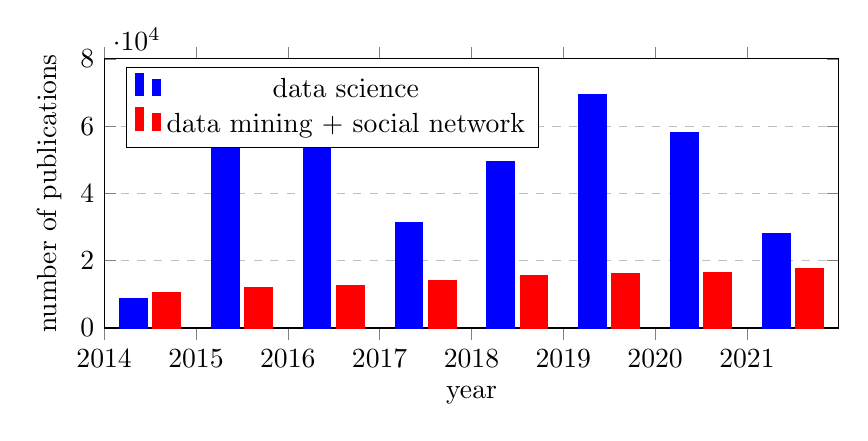
\begin{tikzpicture}
\begin{axis}[
	/pgf/number format/1000 sep={},
	ybar,bar width=10pt,
    xlabel={year},
    ylabel={number of publications},
    xmin=2014, xmax=2022,
    ymin=0, ymax=80000,
    xtick={2012,2013,2014,2015,2016,2017,2018,2019,2020,2021},
    ytick={0,20000,40000,60000,80000,100000,120000,140000,160000,180000},
    legend pos=north west,
    ymajorgrids=true,
    grid style=dashed,
    height=5cm,
    width=0.9\textwidth
    ]

\addplot+[ybar,
    color=blue
    ]
    coordinates {
    (2021.5,28000)(2020.5,58000)(2019.5,69500)(2018.5,49500)(2017.5,31200)(2016.5,62800)(2015.5,65800)(2014.5,8900)
    };

\addplot+[ybar,
    color=red
    ]
    coordinates {
    (2021.5,17800)(2020.5,16500)(2019.5,16200)(2018.5,15500)(2017.5,14200)(2016.5,12700)(2015.5,11900)(2014.5,10600)
    };
    \legend{data science,data mining + social network}
\end{axis}
\end{tikzpicture}
\caption{Number of released papers with specific keywords per year}
\label{fig:released_papers_sndm}
\end{figure}

\subsection{Semantic Data Processing}

The topic of sentence segmentation and tokenization has been subject of increased attention for the past years.
From the analysis presented in figure \ref{fig:released_papers_sdp} we can steadily growing academic production, albeit with an overall small production volume.

We ascertain that this is due to the afterthought that sentence segmentation can be in more sophisticated machine learning system, which may reduce it's overall interest when compared with other language processing topics.

Regarding feature selection, we include an initial term in order to properly filter out ambiguity from other fields with similar terminology. With this, we also find that feature selection still plays an important and growing field in natural language processing, at a greater scale than sentence segmentation.

\begin{figure}[htb]
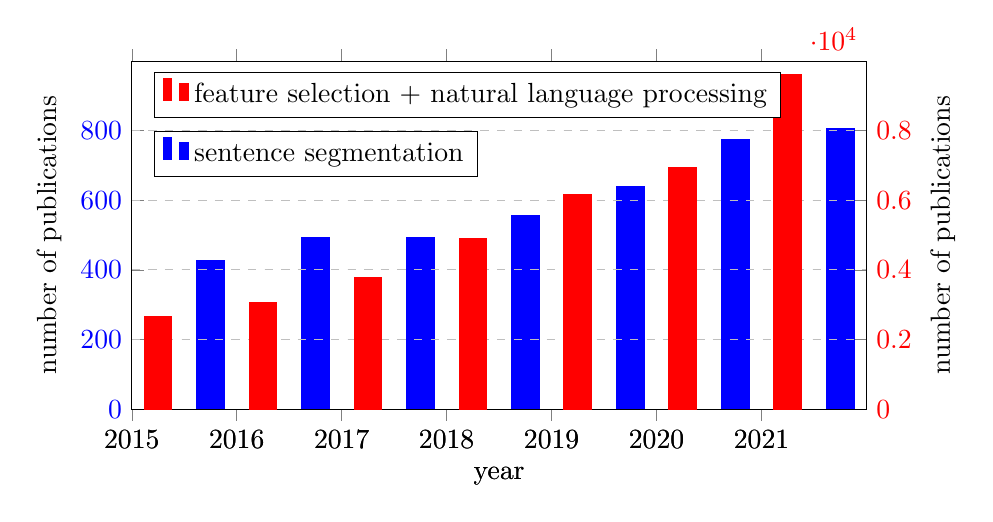
\begin{tikzpicture}
\begin{axis}[
	/pgf/number format/1000 sep={},
	ybar,bar width=10pt,
    xlabel={year},
    y tick label style={blue},
    ylabel={number of publications},
    xmin=2015, xmax=2022,
    ymin=0, ymax=1000,
    xtick={2015,2016,2017,2018,2019,2020,2021},
    ytick={0,200,400,600,800},
    legend pos=north west,
    ymajorgrids=true,
	legend style= {at={(0.03,0.8)}},
    grid style=dashed,
    height=6cm,
    width=0.9\textwidth
    ]

\addplot+[ybar,
    color=blue
    ]
    coordinates {
    (2021.75,806)(2020.75,774)(2019.75,641)(2018.75,557)(2017.75,493)(2016.75,492)(2015.75,427)
    };
    \legend{sentence segmentation}
\end{axis}
\begin{axis}[
	/pgf/number format/1000 sep={},
	ybar,bar width=10pt,
    xlabel={year},
    axis y line*=right,
    y tick label style={red},
    ylabel={number of publications},
    xmin=2015, xmax=2022,
    ymin=0, ymax=10000,
    xtick={2015,2016,2017,2018,2019,2020,2021},
    ytick={0,2000,4000,6000,8000},
    legend pos=north west,
    ymajorgrids=true,
    grid style=dashed,
    height=6cm,
    width=0.9\textwidth
    ]
\addplot+[ybar,
    color=red
    ]
    coordinates {
    (2021.25,9630)(2020.25,6930)(2019.25,6180)(2018.25,4900)(2017.25,3780)(2016.25,3050)(2015.25,2670)
    };
    \legend{feature selection + natural language processing}
\end{axis}
\end{tikzpicture}
\caption{Number of released papers with specific keywords per year}
\label{fig:released_papers_sdp}
\end{figure}

\subsection{Sentiment Analysis}

Sentiment analysis is a popular topic for research throughout the years, as we can see in figure \ref{fig:released_papers_sa}. This graph show us that interest and research into this topic has been steady for the last decade, mostly due to the maturity of this field.

\begin{figure}[htb]
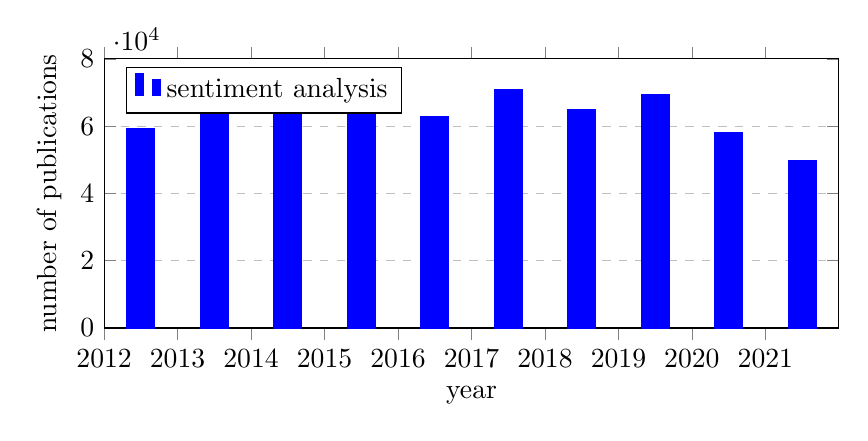
\begin{tikzpicture}
\begin{axis}[
	/pgf/number format/1000 sep={},
	ybar,bar width=10pt,
    xlabel={year},
    ylabel={number of publications},
    xmin=2012, xmax=2022,
    ymin=0, ymax=80000,
    xtick={2012,2013,2014,2015,2016,2017,2018,2019,2020,2021},
    ytick={0,20000,40000,60000,80000,100000,120000,140000,160000,180000},
    legend pos=north west,
    ymajorgrids=true,
    grid style=dashed,
    height=5cm,
    width=0.9\textwidth
    ]

\addplot+[ybar,
    color=blue
    ]
    coordinates {
    (2021.5,49800)(2020.5,58000)(2019.5,69500)(2018.5,64800)(2017.5,70800)(2016.5,62800)(2015.5,65800)(2014.5,65100)(2013.5,67900)(2012.5,59300)
    };
    \legend{sentiment analysis}
\end{axis}
\end{tikzpicture}
\caption{Number of released papers with specific keywords per year}
\label{fig:released_papers_sa}
\end{figure}

\section{State of the Art}

\subsection{Social Network Data Mining}

The size of the data at our disposal and its generation speed is too big to fit in structures of generic existing database architectures in such a way that must be different ways to oversee it \cite{Tappe2016AnalysisAD}.

Predictive tasks of data mining include Classification, Regression and Deviation Detection. Descriptive tasks include Clustering, Summarization, Connection Learning and Sequential Patterns. Clustering or unconfirmed learning is an important but difficult problem; the impartial of clustering is to partition a set of unlabelled objects into standardized groups or clusters. 

Clustering is a process to automatically divide volumes of data into groups that are related to each other on a basis of common themes or properties – to find out what a collection contains. It is applied to identify properties of a set of data as date, cost, etc., and divide them into clusters. Clusters or subsets can be used to find hidden similarities \cite{Kendi2018SocialMM}.

Many clustering techniques are used by applications to establish or realizing structure in data, such as data mining information retrieval image subdivision and machine learning; as a result, clusters of data can be appeared with dissimilar figures, magnitudes, data scarceness and grades of split-up \cite{Tappe2016AnalysisAD}. All these complexities introduce noise in the data and can mask the true nature of the structure of data.

Data mining and Natural Language Processing are interlinked in a way that one extends the analysis of data the extraordinary field of comprehension of data. Romero and Ventura established this relation that emerging text mining technology attempt to extract meaningful information from unstructured textual data. Text mining can be used to identify efficiently and systematically, extract, manage, integrate, and explore knowledge from texts \cite{Kendi2018SocialMM} \cite{article}. As an example, the most important difference between naïve Bayes and logistic regression is that logistic regression is a discriminative classifier while naïve Bayes is a generative classifier, meaning a generative model would have the goal of understanding what dogs look like and what cats look like – by contrast, a discriminative model is only trying to learn to distinguish the classes and perhaps without learning much about them. All the dogs in the training set wear collars and cats not \cite{INJADAT2016654}.

During a detailed survey about data mining techniques used in social media, investigators of Western Ontario and Sharjah Universities performed a deep exploration, including the percentages of data mining types applied with artificial intelligence algorithms by researchers in social media. Technique list below.

\begin{itemize}
	\item AdaBoost
	\item Artificial Neural Networks (ANN)
	\item Apriori
	\item Bayesian Networks (BN)
	\item Decision Trees (DT)
	\item Density Based Algorithm (DBA)
	\item Fuzzy
	\item Generic Algorithm (GA)
	\item Hierarchical Clustering (HC) 
	\item K-Means
	\item K-nearest Neighbors (k-NN)
	\item Linear Discriminant Analysis (LDA)
	\item Linear-Regression (Lin-R)
	\item Logistic Regression (LR)
	\item Markov
	\item Maximum Entropy (ME)
	\item Novel
	\item Support Vector Machines (SVM)
	\item Wrapper
\end{itemize}

\begin{figure}[htb]
	\centering
	\includegraphics[width=.6\textwidth]{images/Picture1.png}
	\caption{Data Mining Techniques among selected papers}
	\label{fig:figure1}
\end{figure}


\subsection{Semantic Data Processing}

An extensive word list combined with an informed segmentation algorithm can help to achieve a certain degree of accuracy in word segmentation, but the greatest barrier to accurate word segmentation is in recognizing unknown words, words not in the lexicon of the segmenter. This problem is dependent both on the source of the lexicon as well as the correspondence (in vocabulary) between the text in question and the lexicon. Another obstacle to high-accuracy word segmentation is the fact that there are no widely-accepted guidelines as to what constitutes a word, and there is therefore no agreement on how to “correctly” segment a text in an unsegmented language. Native speakers of a language do not always agree about the “correct” segmentation, and the same text could be segmented into several very different (and equally correct) sets of words by different native speakers. A simple word segmentation algorithm is to consider each character a distinct word. This is a practical for Chinese because the average word length is very short (usually between one and two characters, depending on the corpus) and actual words can be recognized with this algorithm. Although it does not assist in tasks such as parsing, part-of-speech tagging, or text-to-speech systems, the character-as-word segmentation algorithm has been used to obtain good performance in Chinese information retrieval, a task in which the words in a text, play a major role in indexing.

A very common approach to word segmentation is to use a variation of the maximum matching algorithm, frequently referred to as the greedy algorithm. 
The greedy algorithm starts at the first character in a text and, using a word list for the language being segmented, attempts to find the longest word in the list starting with that character. If a word is found, the maximum-matching algorithm marks a boundary at the end of the longest word, then begins the same longest match search starting at the character following the match.
If no match is found in the word list, the greedy algorithm simply segments that character as a word (as in the character-as-word algorithm above) and begins the search starting at the next character. 

Successful high-accuracy segmentation requires a thorough knowledge of the lexical and morphological features of the language. Languages like Japanese and Korean have writing systems that incorporate alphabetic, syllabic and logo-graphic symbols. Modern Japanese texts, for example, frequently consist of many different writing systems: Kanji (Chinese symbols), hiragana (a syllabary for grammatical markers and for words of Japanese origin), katakana (a syllabary for words of foreign origin), romanji (words written in the Roman alphabet), Arabic numerals, and various punctuation symbols. 
In some ways, the multiple character sets make tokenisation easier, as transitions between character sets give valuable information about word boundaries.


\subsection{Sentiment Analysis}

\subsubsection{Valence Aware Dictionary for sEntiment Reasoning (VADER)}

An example of a state of art model that had impact in sentiment analysis field is the Valence Aware Dictionary for sEntiment Reasoning (VADER), which is a rule-based model for general sentiment analysis. VADER outperformed previous Sentiment Analysis models such as LIWC, ANEW, the General Inquirer and SentiWordNet \cite{Hutto_Gilbert_2014}, especially in text extracted from Social Networks. In contrast to the previous sentiment analysis models, VADER can interpret accurately the sentiment of some common slang and emojis, which increases the performance of sentiment analysis, especially in informal environments such as social networks. 

VADER uses five different heuristics to measure the sentiment of sentences: 

\begin{itemize}
	\item Punctuation: the type and amount of punctuation has a direct impact in the sentiment of the sentence. For instance, “4.0 Industry is cool!!!” has a more positive sentiment than “4.0 Industry is cool” 
	\item Capitalization: if a word is in capital letters, the sentiment is higher, therefore it should have a higher impact in the overall sentiment of the phrase. Example: “The traffic today was HORRIBLE” was a worst sentiment than having the word “horrible” in lower case 
	\item Degree Modifiers (intensifiers or booster words): take in consideration the words before a word that has positive or negative impact in the sentence. For instance, if someone describes something as “incredibly good”, the sentiment is way more positive than having “kind of good”
	\item Contrastive conjunction “but”: usually when a sentence is divided by a “but” word, the dominant sentiment is in the second part of the sentence. VADER reduces up to 50\% the value of sentiment before the “but”, while those after increase to 150\% the value of the sentiment \cite{Calderon_2018}. For instance: “I love the new iPhone but the battery is weak” 
	\item Examining the tri-gram preceding a sentiment-laden lexical feature: heuristic used to find negated sentences that flip the polarity of the sentence. If a negation is captured, VADER multiplies the sentiment of the sentence by -0.74. Example of negated sentence that flips the polarity: “The food here isn’t really all that great” \cite{Hutto_Gilbert_2014}
\end{itemize}
 

Using these heuristics, VADER was able to similar results than individual humans rating the sentiment of text tweets. In those tests, r(correlation to ground truth, mean of 20 human raters) for VADER was = 0.881 while the r for individual humans was 0.888 \cite{Hutto_Gilbert_2014}.  

\subsubsection{TextBlob} is a textual processing Python library capable of doing different tasks such as: 

\begin{itemize}
	\item Noun phrase extraction 
	\item Part-of-speech tagging 
	\item Sentiment analysis 
	\item Classification (Naive Bayes, Decision Tree) 
	\item Tokenization (splitting text into words and sentences) 
	\item Word and phrase frequencies 
	\item Parsing 
	\item n-grams 
	\item Word inflection (pluralization and singularization) and lemmatization 
	\item Spelling correction 
	\item Add new models or languages through extensions 
	\item WordNet integration 
\end{itemize}
 

The sentiment property output given by TextBlob returns a tuple that contains both the polarity, which is the sentiment of the sentence, which ranges from -1 to 1 and subjectivity, which is are the personal feelings, which range from 0 to 1, where 0 is very objective and 1 very subjective. 

TextBlob was built based on NLTK and Pattern, also providing many of the native features \cite{loria2018textblob}.

\section{Applications}

\subsection{Social Network Data Mining in Marketing and Quality Control}

Data mining is a mature technology and currently widespread and used across many distinct industries in a regular basis. Retail stores, hospital, banks, and insurance companies are among the many using it to feed the mechanics of their decision processes. “Data mining has wide application domain almost in every industry where the data is generated that’s why data mining is considered one of the most important frontiers in database and information systems” \cite{Bharati}, Organizations combine data mining with statistics, pattern recognition, and other important tools to find patterns and connections that would otherwise be difficult to find. Data mining allows them to learn more about their customers and users as well as their competitors in a way they can make smart marketing decisions.

Artificial intelligence applied to Data Mining introduced techniques that use information and knowledge intelligently; research categories like Neural networks; Algorithm architecture; Dynamic prediction based approaches; Analysis of systems architecture; Intelligence agent systems; Modelling and its applications; Knowledge-based systems; Systems optimizations; Information systems \cite{liao}.

Practical examples of data mining applied to marketing but not exclusively:

\begin{itemize}
	\item FBTO Dutch Insurance Company, challenged to reduce email costs; increase efficiency of marketing campaigns and increase cross-selling to existing customers – resulted in marketing team with new capabilities to predict the effectiveness of its campaigns; increased efficiency of marketing campaign creation, optimization, and execution. Decreased mailing costs by thirty five percent and increased conversion rates by forty percent.
	\item In 2017 the Journal of Advertising published a study about the utilization of social media mining techniques to gauge users’ perception of a variety of brands. Twitter feed API was used over a six-month period to examine tweets about different stores, telecoms, consumer electronics and footwear companies. The data was collected, compiled, and boil down to a general topic and sentiment with very specific results. Circa fifteen percent of tweets about fast-food restaurants were about promotions and sixty six percent of tweets expressing negative sentiment about Comcast company \cite{McCourt_2018}.
	\item The ability to continually change and provide new understanding is the principal advantage of Data Mining and will be the core of Data Mining applications in future \cite{liao}. This means that whenever possible, Data Mining will be applied to help decision makers take the knowledge one step further by learning with new data structures and patterns.
\end{itemize}

\subsection{Sentiment Analysis in Marketing and Quality Control}

It is important to consider consumers’ opinions on any product, however, surveys can lead to abstract ratings. A better way to obtain a consumer’s opinion is through sentiment analysis on social networks. 
There are various applications for Sentiment Analysis:

\begin{itemize}
	\item Hotel reviews \cite{inproceedings}
	\item Restaurant reviews \cite{doi:10.1080/1528008X.2016.1250243} \cite{10.1007/978-981-13-5802-9_60}
	\item Stock price prediction \cite{Liu_Lu_du_2019}
\end{itemize}

Sentiment analysis has been used to automatically classify consumer comments concerning marketing 4Cs aspects (customer, cost, convenience, communication) \cite{LIN2020106755}. 

During the COVID-19 pandemic, some papers also suggested the use of Sentiment Analysis in order to better understand the pandemic effects on subjects such as vaccine rejection and false information spread. Some papers suggest a deeper study of the impact of the pandemic through Sentiment Analysis in order to be better prepared for the next one \cite{ALAMOODI2021114155}.

\bibliography{refs}

\end{document}